\chapter{\textbf{REFERENCIAL TEÓRICO}}

\section{\textbf{Saneantes versus SARS-CoV-2}}

O novo coronavírus, conforme é demonstrado na Figura \ref{fig:acaoforcasintermoleculares} \cite{lima2020quimica}, ocasionando então a destabilização seguido da separação ou rompimento da membrana que leva a liberação do conteúdo intracelular causando a morte do vírus.

%EXEMPLO FIGURA
\begin{figure}[htb!]
	   \centering
	   \caption{Esquema da ação do tensoativo por meio das forças intermoleculares}
	   		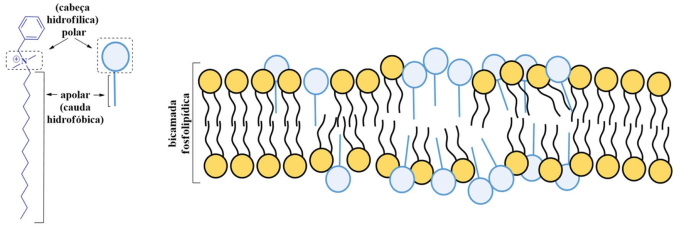
\includegraphics[scale=0.8]{04-figuras/acaoforcasintermoleculares.png}
	   	    \fonte{\citeonline{daltin2011tensoativos} } \label{fig:acaoforcasintermoleculares}
\end{figure}


\subsection{Definição}

Tensoativo (ou surfactante) ...
   
